\section{Compiler}\label{sec:compiler}

Damit eine Programmiersprache verwendbar ist, muss sie nicht nur eine Spezifikation haben, sondern auch ausführbar sein.
Dies kann durch direktes Ausführen des Programmtexts geschehen;
in diesem Fall wird das ausführende Programm Interpreter genannt.
FulibScenarios verwendet jedoch den zweiten Ansatz der Kompilierung.
Dabei werden die vorliegenden Quelltexte zunächst in eine andere Text- oder Binärsprache übersetzt.
Ziel der Kompilierung von FulibScenarios sind Java-Quelltextdateien.
Die Übersetzung von Markdown-Scenario-Quelltexte in Java-Quelltexte wird durch den Scenario-Compiler durchgeführt.
Dessen Architektur und Implementierung sind Inhalt dieses Abschnitts.
Dabei wird des öfteren auf das Beispiel in Listing~\ref{lst:CompilationExample.md} Bezug genommen, dessen Übersetzung in den einzelnen Teilabschnitten stückweise erarbeitet wird:

% TODO markdown
\codelisting{text}{chapter/fulib-scenarios/scenarios}{CompilationExample.md}{Beispiel-Szenario für diesen Abschnitt}

\subsection{Architektur}\label{subsec:compiler-architecture}

\todo{
Visitor Pattern~\cite{gof-design-patterns}.
Dragon Book~\cite{dragonbook}.
}

\begin{figure}
	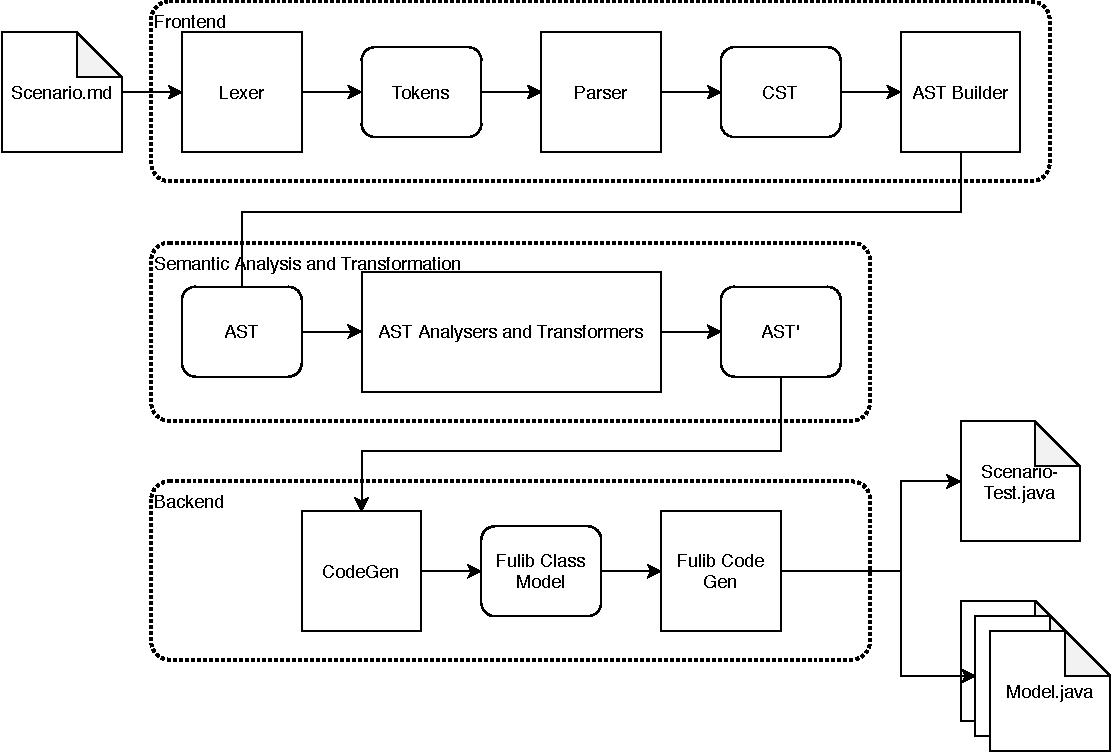
\includegraphics[width=\textwidth]{chapter/fulib-scenarios/img/architecture.pdf}
	\caption{Compiler-Architektur}
	\label{fig:compiler-architecture}
\end{figure}

\subsection{Frontend - ANTLR v4}\label{subsec:frontend-antlr4}

\todo{
Warum ANTLR4 sehr gut für die Sprachstruktur geeignet ist~\cite{adaptive-ll-star,antlr4-reference}.
}

\subsection{AST, Analyse und Transformation}\label{subsec:data-model-gentreesrc}

\todo{
AST mit GenTreeSrc;
eigenes Projekt, kurze Erklärung.
Prä-Transformation: Gruppieren von Sätzen zu Methoden
Analyse: Variablen, Konflikte bei Attributen und Assoziationen, Programmstruktur.
Transformation: Bauen von Klassenmodell, Vereinfachung des AST in Vorbereitung auf CodeGen.
}

\subsection{Codegenerierung - Fulib}\label{subsec:codegen-fulib}

\todo{
Modellgenerierung mit Fulib.
Testgenerierung selbst.
}
